\section{Empirical Test: The Onset Structure (E5)}
\label{sec:supp-e5}

\subsection{Empirical test: the onset structure (E5)}\label{sec:e5}

E5 places Theorem~\ref{thm:onset} on constructed planes with known onset:
the attacker-tomographer either memorizes a pre-onset reference batch of
size $N_0$ or has none (birth onset), and we track the AUC of its
two-sample detection statistic as the fresh-sample horizon $M$ grows ($120$
trials per point; event rate $p=0.30$; frozen world data). This section
reports a \emph{falsified registration and a post hoc reading}, in that
order, because that is what the frozen record contains.

\paragraph{The registered prediction, and why it failed}
The E5 registration (\texttt{PREREGISTRATION\_E2E3.md} \S E5, commit
preceding driver and data) predicted, verbatim: ``(a) detection advantage
$\to1$ for $\delta$ above the reference noise floor, (b) flat at chance
$\forall M$.'' The frozen data falsify that prediction at three of its
four test points:
\begin{itemize}[leftmargin=1.6em,itemsep=1pt,topsep=2pt]
\item (a) at $(N_0,\delta)=(10,0.4)$---above the floor---the AUC runs
$0.909/0.965/0.928/0.935$ over $M=5/10/20/40$: a non-monotone plateau
$0.91$--$0.97$ that never approaches $1$;
\item (a) at $(40,0.2)$ rises $0.760/0.861/0.913/0.967$---advantage grows
but stops at $0.97$;
\item (b) fails in both directions: the below-floor known-onset cell
$(10,0.2)$ is flat at $0.69$--$0.74$, i.e.\ flat \emph{but} $19$--$24$
AUC points \emph{above} chance; and the birth-onset self-tests read
$0.431$--$0.529$ at $\delta=0.2$ (two of the four readings below chance)
but $0.339$--$0.439$ at $\delta=0.4$, up to $0.16$ \emph{below} chance.
\end{itemize}
Only $(40,0.4)$ matches the registered form
($0.918/0.997/0.997/1.000$). Theoretical reading, in arrears: the data
showed the \emph{earlier draft's} statement of this theorem---which
printed $\delta\ge\rho_0$ as sufficient for certified detection---to be
false as algebra, since at $\delta=\rho_0$ the limiting power is
$\Phi(0)=0.50$; the corrected boundary $\Delta_{\beta_d}=1.84\,\rho_0$ and
the three-regime statement above follow from that computation, and E5's
middle-cell plateaus are consistent with them. The two middle cells sit exactly where the
corrected theorem puts them: $\delta/\sigma_0=2.76<3.6$, so certified
power is unattainable at \emph{every} horizon (limiting power
$\Phi(0.80)=0.79$; the exact one-sided binomial test at level $\beta_d$ on
the $N_0$ draws gives $0.850$ at $(10,0.4)$ and $0.785$ at $(40,0.2)$). This is the plateau the
registration read as a failure of its own prediction (a). The E5 run's
verdict gate compounded the miss: it tested the advantage arm only at the
safest cell $(40,0.4)$ and the birth arm only \emph{against}
above-chance exceedance---a one-sided criterion that could not see the
below-chance birth readings; \texttt{E5\_ONSET.md}'s ``dichotomy
manifests'' verdict is superseded by the falsification reading here, and
the run's result was logged, post-data, inside the registration file's
deviation log (pinned as frozen in the claims--evidence ledger; Data
Availability). E5 has no frozen-twin registration copy; its birth-onset
readings are \emph{descriptive statistics against
Remark~\ref{rem:birth}}, not a test of it.

\begin{figure}[t]
\centering
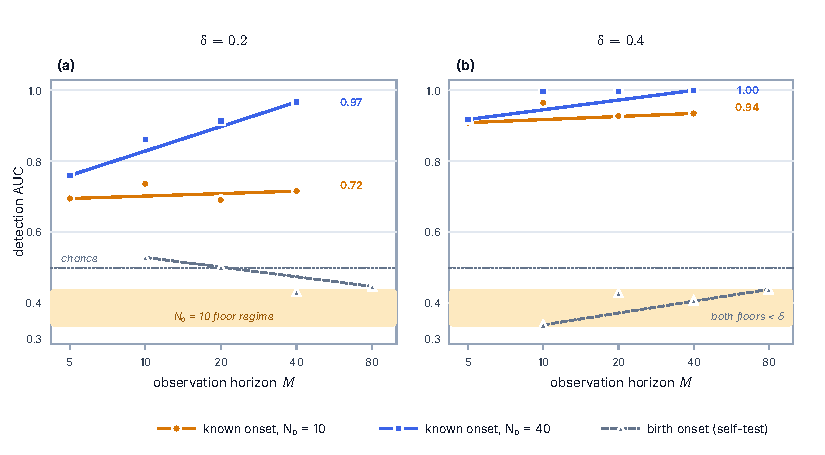
\includegraphics[width=\columnwidth]{anthro/fig2_onset.pdf}
\Description{Two panels, one per deception footprint, plotting detection
AUC against the observation horizon on a log scale. Two solid curves for a
known-onset attacker with 10 and 40 memorized reference turns rise to
plateaus of different heights, one pair saturating near one and the other
pair stalling in the 0.7 to 0.97 range. A dashed birth-onset curve
oscillates slightly below the chance line at every horizon.}
\caption{E5: onset regimes on constructed planes (all frozen values).
Detection AUC of the two-sample statistic vs.\ fresh-sample horizon $M$;
one panel per footprint $\delta$. Solid curves memorize a reference batch
($N_0=10$, $N_0=40$); the dashed curve is the birth-onset self-test
($N_0=0$), whose registered ``flat at chance'' prediction failed: it reads
$0.431$--$0.529$ at $\delta=0.2$ (two of the four readings below chance)
and $0.339$--$0.439$ at $\delta=0.4$,
up to $0.16$ \emph{below} chance (a small-sample asymmetry of the
studentized statistic: with $N_0=0$ the reference stream doubles as the
first half of the $M$-sample draw, so the lattice of the score's null
distribution sits a half step below chance at short $M$, and the
plug-in variance from the same path is conservative by design of the
two-sample plug-in). Plateaus: $(10,0.2)$ flat at
$0.69$--$0.74$, $19$--$24$ points above chance; $(40,0.2)$ rising to
$0.97$; $(10,0.4)$ non-monotone $0.91$--$0.97$; $(40,0.4)$ $0.92\to1.000$.
The corrected boundary $\Delta_{\beta_d}=1.84\rho_0$ orders the extremes;
the shaded band marks the $N_0=10$ reference-width regime.}
\label{fig:onset}
\end{figure}

\paragraph{The post hoc ordinal reading (exploratory)}
Figure~\ref{fig:onset} plots the frozen cells, and Table~\ref{tab:widths}
reads them against the \emph{corrected} boundaries---labeled post hoc
because neither the corrected boundary nor the ordinal comparison appears
in the registration: the registered floors are
$\rho_0=0.284$ and $0.142$ at $N_0=10$ and $40$ ($z=1.96$, $p=0.30$; the
earlier draft printed $0.283/0.141$), the certified boundaries are
$\Delta_{\beta_d}=0.522$ and $0.261$, and the non-adaptive width
$w_{\mathrm{na}}=0.774/0.387$ bounds what a threshold fixed independently
of the honest rate can reach. The reading is qualitative at the middle
cells: $\Delta_{\beta_d}$ orders the extremes (the below-width cell is
capped and lowest; the certified cell alone reaches $1.000$, with
$M^{*}\approx30$ and AUC saturation preceding the certified-power
threshold because AUC pools all thresholds), but the two middle cells'
plateaus overlap ($0.76\to0.97$ rising vs.\ $0.91$--$0.97$ non-monotone)
and admit no strict ordinal claim. The adaptive minimax boundary between
the regimes remains open (Section~\ref{sec:discussion}). The instrument
any reviewer can rerun did its job: it falsified the registered
prediction at three cells, falsified the earlier draft's statement of
this theorem at the middle cells, and now anchors a corrected statement
whose certified horizon matches the only cell that saturates.

\begin{table}[t]\centering\scriptsize
\setlength{\tabcolsep}{3.5pt}
\begin{tabular}{@{}ccccc@{}}
\toprule
$(N_0,\delta)$ & $\rho_0$ & $\Delta_{\beta_d}$ &
regime (restated Thm.~\ref{thm:onset}) & observed AUC (all $M$) \\
\midrule
$(10,0.2)$ & 0.284 & 0.522 & below width & $0.69$--$0.74$, flat \\
$(40,0.2)$ & 0.142 & 0.261 & middle & $0.76\to0.97$ \\
$(10,0.4)$ & 0.284 & 0.522 & middle & $0.91$--$0.97$, non-mon. \\
$(40,0.4)$ & 0.142 & 0.261 & certified & $0.92\to1.000$ \\
\bottomrule
\end{tabular}
\caption{The registered E5 prediction versus the corrected boundaries
(exploratory, post hoc; $\beta_d=0.05$ two-sided; $p=0.30$;
$\rho_0=z_{1-\beta_d/2}\sqrt{p(1-p)/N_0}=0.284/0.142$;
$\Delta_{\beta_d}=(z_{1-\beta_d/2}+z_{1-\beta_d})\sigma_0=1.84\rho_0=0.522/0.261$;
non-adaptive width at one-sided level $\beta_d$,
$w_{\mathrm{na}}=\sqrt{2\ln(1/\beta_d)/N_0}=0.774/0.387$;
observed values frozen, all four $M$ points per cell; regime tokens: below
width (shift capped at $L\rho_0$), middle (uncertified power at every $M$),
certified ($M^{*}\!\approx\!30$)). The registered
prediction (``advantage $\to1$ above the floor; flat at chance'') failed
at three cells (Section~\ref{sec:e5}); the corrected trichotomy orders the
extremes and leaves the two middle cells overlapping plateaus below
certified power (limiting TPR $0.79$ normal; the one-sided exact binomial
test has power $0.850$ at $(10,0.4)$ and $0.785$ at $(40,0.2)$).}
\label{tab:widths}
\end{table}
